%\textsl{}%!TEX TS-options = --shell-escape
%!TEX TS-program = pdflatex
\documentclass[%
   10pt,              % Schriftgroesse
   nenglish,           % wird an andere Pakete weitergereicht
   a4paper,           % Seitengroesse
   DIV11,             % Textbereichsgroesse (siehe Koma Skript Dokumentation !)
]{scrartcl}%     Klassen: scrartcl, scrreprt, scrbook, article
% -------------------------------------------------------------------------

\usepackage[utf8]{inputenc} % Font Encoding, benoetigt fuer Umlaute
\usepackage[english]{babel}   % \textsl{}Spracheinstellung

\usepackage[T1]{fontenc} % T1 Schrift Encoding
\usepackage{textcomp}    % Zusatzliche Symbole (Text Companion font extension)
\usepackage{lmodern,dsfont}     % Latin Modern Schrift
\usepackage{dsfont}
\usepackage{color}
%\usepackage{wasysym}
\usepackage{ulem}
\usepackage{graphicx}
\usepackage{grffile} %allows to use pngs
\usepackage{eurosym}
%\usepackage{txfonts}
\usepackage{stmaryrd}
\usepackage{amsfonts}
\usepackage{amsmath}
\usepackage{hyperref}
\usepackage{tikz}
\usepackage{multirow}
\usepackage{listings}
\usepackage{etextools}
\usepackage{ifthen}
\usepackage{cite}
%\usepackage{TikZ} %phylogenetischer Baum
%\usetikzlibrary{calc, shapes, backgrounds} %für die Phylogenetische bäume
%\usetikzlibrary{automata,arrows}
\usepackage{subfigure} 


% Definition des Headers
\usepackage{geometry}
\geometry{a4paper, top=3cm, left=3cm, right=3cm, bottom=3cm, headsep=0mm, footskip=0mm}
\renewcommand{\baselinestretch}{1.3}\normalsize

\def\header#1#2#3#4#5#6#7{\pagestyle{empty}
\noindent
\begin{minipage}[t]{0.6\textwidth}
\begin{flushleft}
\textbf{#4}\\% Fach
#6\\% Semester
Tutor: #2  % Tutor 
\end{flushleft}
\end{minipage}
\begin{minipage}[t]{0.4\textwidth}
\begin{flushright}
\points{#7}% Punktetabelle
\vspace*{0.2cm}
#5%  Names
\end{flushright}
\end{minipage}

\begin{center}
{\Large\textbf{ Assignment #1}} % Blatt

{(Handed in #3)} % Abgabedatum
\end{center}
}

\newenvironment{vartab}[1]
{
    \begin{tabular}{ |c@{} *{#1}{c|} } %\hline
}{
    \end{tabular}
}

\newcommand{\myformat}[1]{& #1}

\newcommand{\entry}[1]{
  \edef\result{\csvloop[\myformat]{#1}}
  \result \\ \hline
}

\newcommand{\numbers}[1]{
  \newcounter{ctra}
\setcounter{ctra}{1}
\whiledo {\value{ctra} < #1}%
{%
  \myformat{\thectra}
  \stepcounter{ctra}%
}
\myformat{\thectra}
}
\newcommand{\emptyLine}[1]{
  \newcounter{ctra1}
\setcounter{ctra}{1}
\whiledo {\value{ctra1} < #1}%
{%
  \myformat{\hspace*{0.5cm}}
  \stepcounter{ctra1}%
}
}

\newcommand{\points}[1]{
\newcounter{colmns}
\setcounter{colmns}{#1}
\stepcounter{colmns}
  \begin{vartab}{\thecolmns}
    \numbers{#1} & $\sum$ (7)\\\hline   %add here Complete number of points ---------------------------
    \emptyLine{\thecolmns}\\
  \end{vartab}
}


\begin{document}
%\header{Blatt}{Tutor}{Abgabedatum}{Vorlesung}{Bearbeiter}{Semester}{Anzahl Aufgaben}
\header{5}{Alexander Seitz}{16. November 2015}{Bioinformatics I}{\\Jonas Ditz \\\& Benjamin Schroeder}{WS 15/16}{4}

\section*{Theoretical Assignment - \textsl{Comparison with at most $l$ mismatches}}

General we are now only looking at the worst case scenario, which means uniform distributed mistmatches in an alignment. Also we only look at $k>=1$, as $k=0$ is in our application not a useful result. Assume two sequences of length t with l mismatches.\\
 Than both sequences contain $l$ tuples of length $\lfloor\frac{t}{l+1}\rfloor$ and one tuple which has a length of maximal $\lfloor\frac{t}{l+1}\rfloor$ . Where $k = \lfloor\frac{t}{l+1}\rfloor$ is the maximal tuple length, possible in sequences.\\
\\
\noindent So both sequences share $l+1$ k-tuples and for each 
$k \le \lfloor\frac{t}{l+1}\rfloor$ they share $(l+1) * \lfloor\frac{\lfloor\frac{t}{l+1}\rfloor}{k}\rfloor$
k-tuples.

\section*{Theoretical Assignment - \textsl{Linear programming by hand}}

The feasible region of this linear program is shown in figure \ref{feasibleRegion}, where the red line 
is constraint 1, green line is constraint 2, constraint 3 is drawn as a blue line and the yellow line 
is constraint 4.

\begin{figure}[ht]
 \centering
 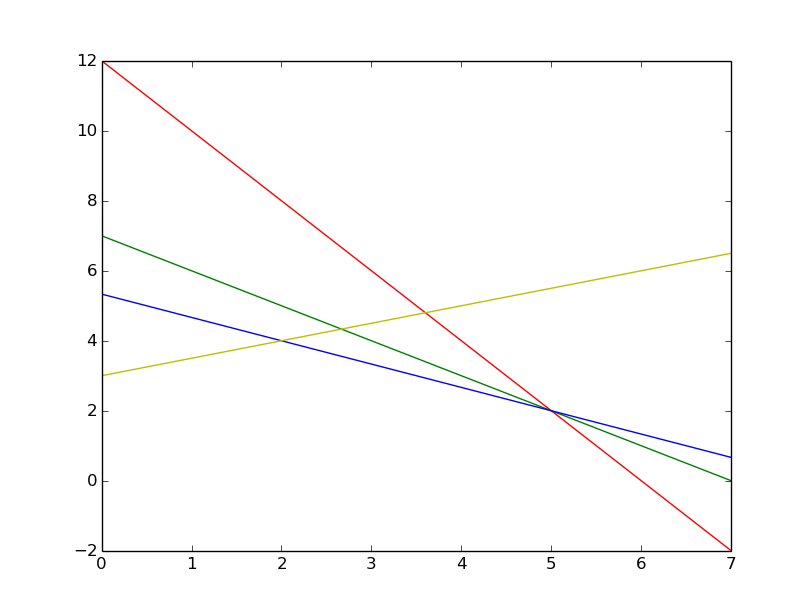
\includegraphics[width=0.7\textwidth]{img/figure_1.png}
 \caption{feasible region of linear program (grey area)}
 \label{feasibleRegion}
\end{figure}

\subsection*{solution if t=s=1}
Generally we only used integers in this task. The constraint for the algorithm are as following if t and s value is 1 now:

\begin{eqnarray}
max: 1*x_1+1*x_2 \label{con1}\\ 
2*x_1+x_2 \le 12 \label{con2}\\ 
2*x_1+3*x_2 \le 7 \label{con3}\\ 
-1*x_1+2*x_2 \le 16 \label{con4}\\ 
x_1,x_2 \ge 0 \label{con5}
\end{eqnarray}

\noindent the next step we started to compute each line of the tuple. Starting with constraint \ref{con3} under the aspect of constraint \ref{con5}. All possible tuples respectively to both constraints from the assignment are:\\
$temp1=\{(0,7);(1,6);(2,5);(3,4);(4,3);(5,2);(6,1);(7,0)\}$\\

\noindent the constraint \ref{con2} was applied to temp1:\\
$temp2=\{(0,7);(1,6);(2,5);(3,4);(4,3);(5,2);\}$\\

\noindent the next constraint (constraint \ref{con4}) was applied:\\
$temp3=\{(5,2)\}$\\

\noindent but not least the last constraint (4) is checked and the remaining tuple from the last step is valid:\\
$r=\{(5,2)\}$\\

\noindent the final result for the Algorithm with s=t=1 is the tuple: (5,2). Solving the formula with this numbers 
leads us to the following maximal value: $1*x_1 + 1*x_2 = 5+2 = 7$\\


\subsection*{How to make unsolvable?}
To get a not solvable algorithm for example the following constraint could be added:
	\begin{equation}\\
		x_1+x_2\ge 7
	\end{equation}

\noindent a new constraint just needs to be a contradiction to another constraint.
	
\subsection*{How to get infinite solutions with t and s?}
The equation influence by t and s is:

\begin{equation*}
max: s*x_1+t*x_2
\end{equation*}

\noindent way to get an infinite solution could be to generate a endless loop with values for s and t like:
\begin{eqnarray*}
s=s*x_1\label{inf1}\\ 
t=t*x_2 \label{inf2}\\ 
or\\
s=t*x_2\label{inf3}\\ 
t=s*x_1 \label{inf4}\\ 
\end{eqnarray*}


\noindent idea of the evening:
Do not assume to only use integers!
Another variant is to define:
\begin{eqnarray*}
	s=\frac{1}{x_1}\\
	t=\frac{1}{x_2}\\ 
\end{eqnarray*}
the result for Z now is 2 and there are infinite many possibilities to get to 2.

\subsection*{how to get the points?}

P1=(0,3)\\
P2=(2,4)\\
P3=(1,3)\\
P4=(6,0)

\section*{Theoretical Assignment - \textsl{Bonus: Carillo-Lipman bound}}

%\newpage
%\bibliography{Assignment4-Ditz_Schroeder-WS15-16.bib}
%\bibliographystyle{ieeetr}
 
\end{document}